\documentclass[a4,12pt]{article}

\usepackage[utf8]{inputenc}
\usepackage[spanish]{babel}
\usepackage[margin=1.5cm]{geometry}
\usepackage{graphicx}
\usepackage{color}
\usepackage{import}
\usepackage{float }



\usepackage{hyperref}

\parindent 0em

%\usepackage{times}
\renewcommand{\familydefault}{\sfdefault}

\title{Resolución de problemas a GNU OCTAVE}
\author{Lamya Hafs}
%\date{}

\begin{document}

\maketitle
\bigskip
\bigskip
\bigskip
\begin{figure}[H]
  \centering
    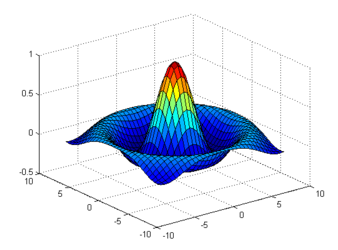
\includegraphics{imagenes/octave}
\end{figure}
\newpage

\maketitle

\begin{abstract}
vacio del momento. Test

\end{abstract}

